For C.8.1, the specified aluminum bar has diameter $D=20.0\,\mathrm{mm}$, Young's modulus $E=70.0\,\mathrm{GPa}$, density $\rho=2700\,\mathrm{kg/m^3}$, and length $L=3.20\,\mathrm{m}$. The slender-bar wave speed from the axial wave equation in the course notes is
\[
c=\sqrt{\frac{E}{\rho}}=\sqrt{\frac{70.0\times10^9}{2700}}
=\boxed{5.09\,\mathrm{km/s}}.
\]

For C.8.2, the one-way pulse travel time is
\[
t=\frac{L}{c}=\frac{3.20}{5091.75}
=\boxed{0.628\,\mathrm{ms}}.
\]

For C.8.3 and C.8.4, the stated bar has no support condition. Taking its ends as free gives $U'(0)=U'(L)=0$. Applying these conditions to $U=C_1\sin\gamma x+C_2\cos\gamma x$ gives $C_1=0$ and $\sin(\gamma L)=0$. The axial bar results in the course notes therefore give $\gamma_j=j\pi/L$, $f_j=jc/(2L)$, and unit-peak displacement $U_j(x)=\cos(j\pi x/L)$ for $j=1,2,3$. The rigid-body mode at zero frequency precedes these elastic modes. For the first elastic mode, $f_1=5091.75/[2(3.20)]=795.6\,\mathrm{Hz}$. The next two are $2f_1$ and $3f_1$. Thus,
\[
\boxed{(f_1,f_2,f_3)=(796,\ 1591,\ 2387)\,\mathrm{Hz}}.
\]
The first three elastic mode shapes are plotted in Figure~\ref{fig:hw03-c8-modes}. These values depend on the assumed free ends.

\begin{figure}[H]
\centering
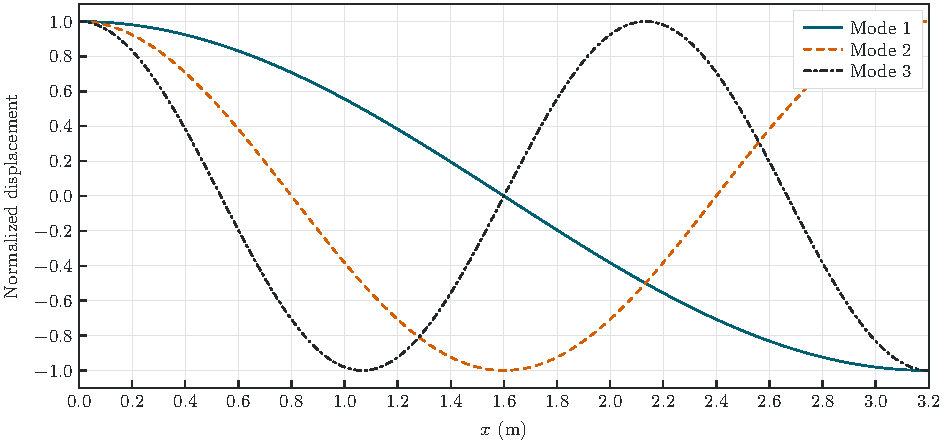
\includegraphics[width=0.90\linewidth]{figures/generated/solutions/C8.pdf}
\caption{Normalized axial displacement modes of the free-free aluminum bar.}
\label{fig:hw03-c8-modes}
\end{figure}

For C.8.5, a split Hopkinson pressure bar, also called a Kolsky bar, tests a specimen between an incident bar and a transmission bar. A striker impacts the incident bar and creates a compressive elastic pulse. At the specimen, part of the pulse reflects into the incident bar and part passes through the specimen into the transmission bar. Strain gauges record the incident, reflected, and transmitted pulses. With appropriate one-dimensional wave analysis, the transmitted pulse gives specimen stress and the reflected pulse gives specimen strain rate. Integrating the strain rate produces strain and hence a high-rate stress--strain response. The method characterizes material behavior at high loading rates, including compression tests on structural alloys. The NIST report describes how the measured pulses are reduced to specimen stress and strain~\cite{Whitenton2005Kolsky}.

\lstinputlisting[style=hwmatlab]{matlab/C8.m}
